\section{Chisel}
\label{sec:chisel}
Chisel is a domain-specific language embedded in the Scala
programming language so it is really just a library of Scala functions
and data structures. Someone writing Chisel code is essentially writing a Scala
program that uses the provided functions and data structures to
construct hardware. This chapter introduces the core
components of the Chisel hardware construction language; readers
interested in a more a detailed specification of Chisel should consult
the Chisel manual. 

\subsection{Node}
Hardware circuits are represented in Chisel as directed graphs of
{\tt Nodes}, which are the base class from which all circuit elements are
derived. Figure~\ref{fig:hier} shows the Chisel class
hierarchy and Figure~\ref{fig:nodeapi} shows the API for the Node class.

{\bf Types}. Chisel has its own type system that is maintained
independent of the Scala type system. Figure~\ref{fig:hier} shows the
Chisel data types and their hierarchy (everything rooted at
{\tt Data}). {\tt Bits} is used to represent raw collection of bits,
{\tt Bool} is used to represent Boolean literals, and {\tt Num} is
used to represent numbers. Note that {\tt Num} has two subclasses,
{\tt Fix} and {\tt UFix} which are used for signed and unsigned
numbers respectively.

\begin{figure}[hb]
\centering
  \begin{subfigure}[t]{0.48\textwidth}
  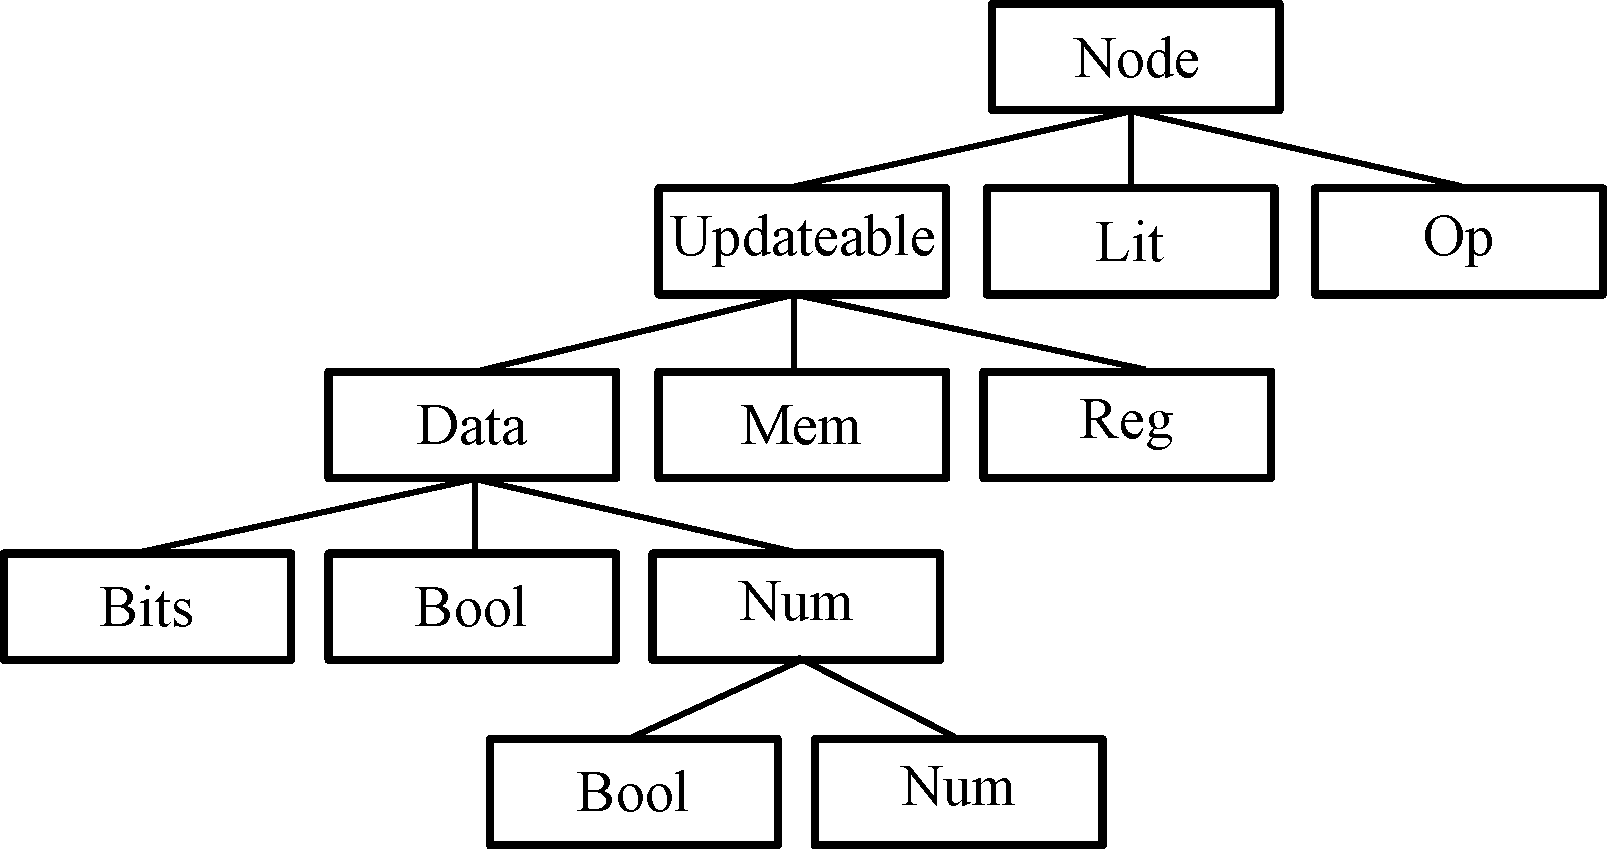
\includegraphics[width=\textwidth]{figures/hierarchy.pdf}
  \caption{Hierarchy}
  \label{fig:hier}
  \end{subfigure}
  \hfill
  \begin{subfigure}[t]{0.48\textwidth}
  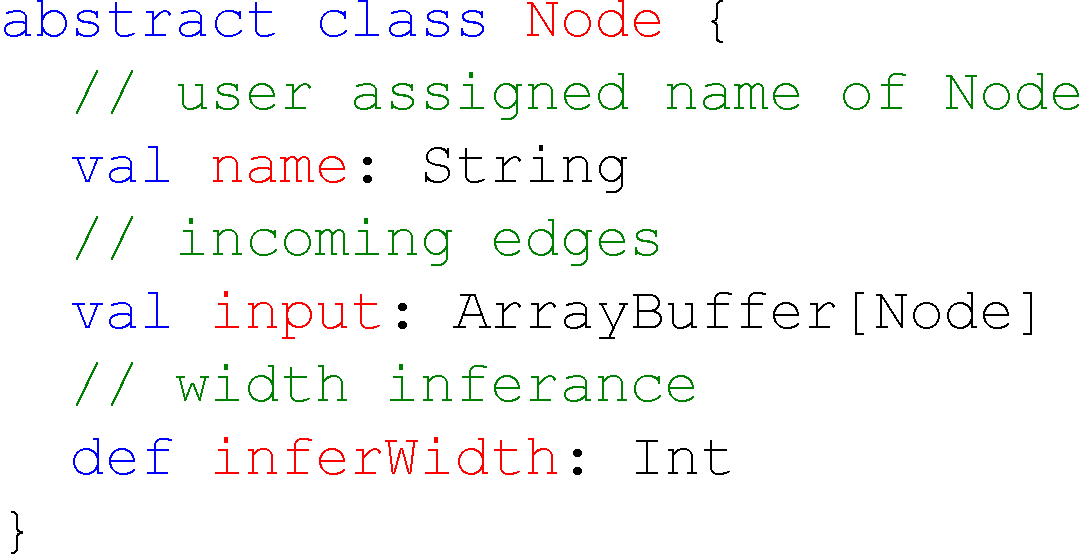
\includegraphics[width=\textwidth]{figures/node.pdf}
  \caption{API}
  \label{fig:nodeapi}
  \end{subfigure}
  \hfill
  \caption{Chisel Node}
  \label{fig:node}
\end{figure}

{\bf Arithmetic and Logic}. Arithmetic and logic operations
are represented with {\tt Op} nodes. The Chisel manual has an
exhaustive list of supported operations. Op nodes are constructed
whenever a user invokes the corresponding type node member
function for the operation. For example, suppose we have two {\tt
Bits} nodes, {\tt a} and {\tt b}, and want to connect them to the
inputs of an AND gate. The Chisel code that will do this is {\tt a \&
b} which is actually syntactic sugar for {\tt a.\&(b)}. The {\tt \&}
function that Bits defines will instantiate an {\tt Op} node to
represent the {\tt \&} and put the two {\tt Bits} nodes, {\tt a} and
{\tt b}, into the {\tt Op} node's input.

The example Chisel code in Figure~\ref{fig:mux} shows Bits nodes and
Op nodes interacting to create a 2-input multiplexor built out of {\tt
\&} and {\tt |} gates. In this example,  {\tt a}, {\tt b}, and {\tt
 sel} are incoming {\tt Bits}. Invoking {\tt a \& sel} will create a
new {\tt Op} and connect that node to a {\tt Bits} since both inputs
are {\tt Bits}. The output of the circuit, {\tt c}, will be the {\tt
Bits} connected to the {\tt |} {\tt Op}. 

\begin{figure}[t]
\centering
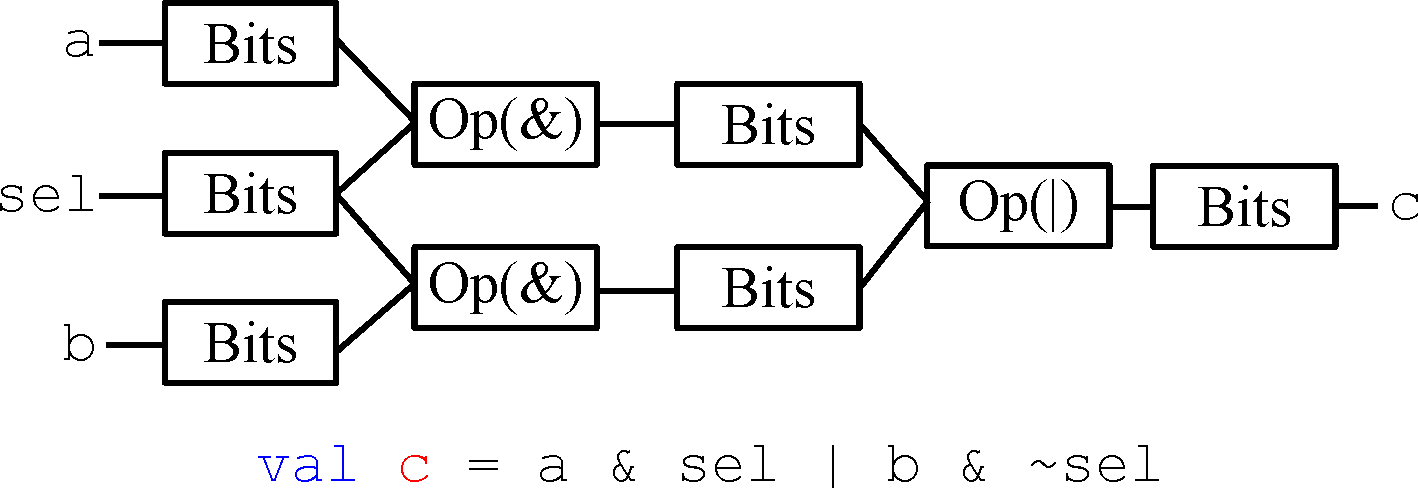
\includegraphics[width=0.75\textwidth]{figures/mux.pdf}
\caption{2-Input Mux}
\label{fig:mux}
\end{figure}

{\bf Literals} The {\tt Lit} node works in conjunction with type {\tt Nodes} to
represent literals. Figure~\ref{fig:lits} shows example Chisel code for
instantiating literals. True and false literals are represented as Bools
connected to {\tt Lit} nodes 1 and 0 respectively. Arbitrary bit
strings can be represented with {\tt Bits} Nodes and numbers can be represented with
{\tt Fix} and {\tt UFix} Nodes, all of which are connected to {\tt Lit
Nodes} with the appropriate value.

\begin{figure}[b]
\centering
  \begin{subfigure}[t]{0.22\textwidth}
  \centering
  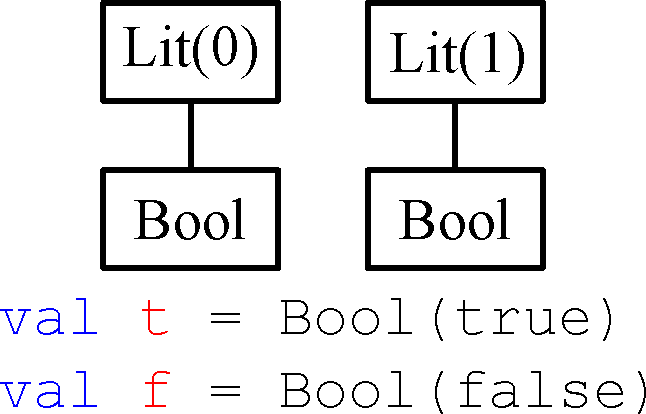
\includegraphics[width=\textwidth]{figures/bool.pdf}
  \caption{Bool literals}
  \label{fig:bool}
  \end{subfigure}
  \hfill
  \begin{subfigure}[t]{0.22\textwidth}
  \centering
  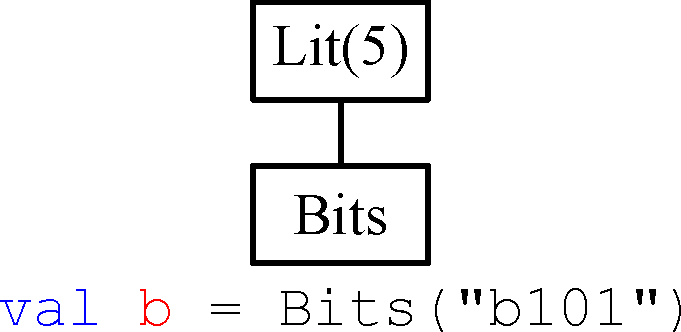
\includegraphics[width=\textwidth]{figures/bits.pdf}
  \caption{Bits literals}
  \label{fig:bits}
  \end{subfigure}
  \hfill
  \begin{subfigure}[t]{0.22\textwidth}
  \centering
  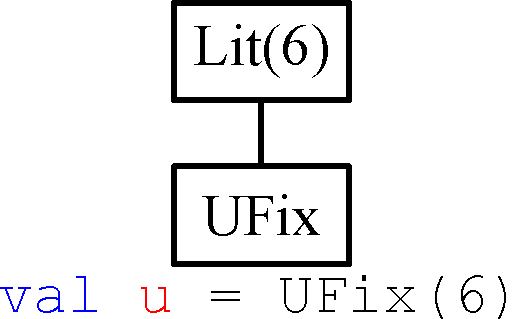
\includegraphics[width=\textwidth]{figures/ufix.pdf}
  \caption{UFix literals}
  \label{fig:ufix}
  \end{subfigure}
  \hfill
  \begin{subfigure}[t]{0.22\textwidth}
  \centering
  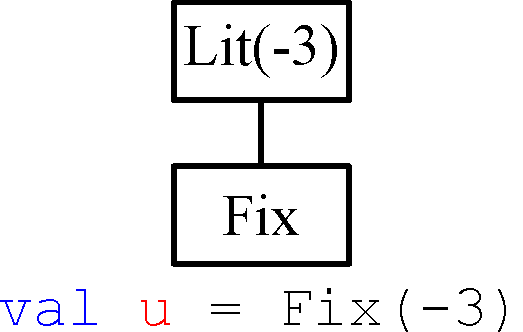
\includegraphics[width=\textwidth]{figures/fix.pdf}
  \caption{Fix literals}
  \label{fig:fix}
  \end{subfigure}
\caption{Chisel Literal Examples}
\label{fig:lits}
\end{figure}

{\bf Registers} The {\tt Reg} node, Chisel most basic state element,
represents a positive-edge-triggered flip-flop. {\tt Reg} nodes, unlike the
previous nodes, are manually instantiated by the user. The manual
details the different ways that a Reg can be constructed. Briefly,
Regs can be constructed either with or without an update signal.
{\tt Reg}'s constructed without an update signal can
be conditionally updated.

{\bf Memories} {\tt Mem Nodes} are used to represent random access
memories. These memories can be accessed with either {\tt Bits} or
{\tt UFix} nodes. Writes to these memories are positive-edge-triggered while
reads can be either combination or positive-edge-triggered.

\subsection{Component}
In addition to {\tt Nodes}, Chisel also provides {\tt Components} to allow users
to organize their directed graph of {\tt Nodes} into subgraphs, adding a
hierarchical structure to their hardware. Figure~\ref{fig:muxcomp} shows an
example of a Chisel implementation of a 4-input mux built from three 2-input muxes.

\begin{figure}
\centering
  \begin{subfigure}[t]{0.48\textwidth}
  \centering
  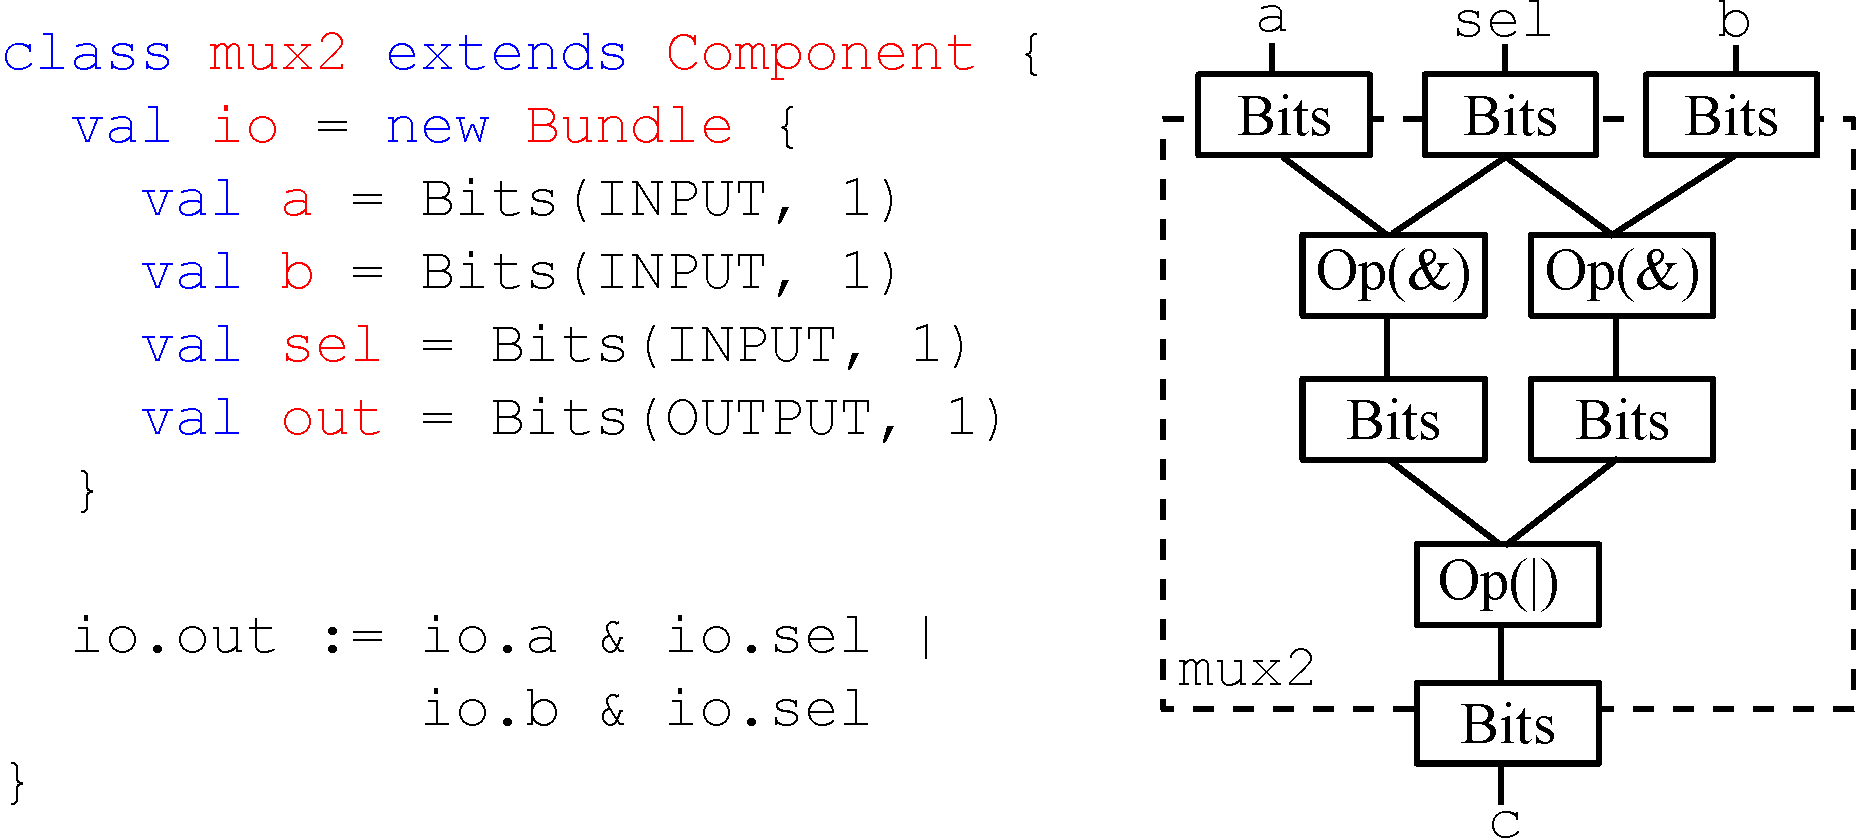
\includegraphics[width=\textwidth]{figures/mux2.pdf}
  \caption{2-Input Mux}
  \label{fig:mux2}
  \end{subfigure}
  \hfill
  \begin{subfigure}[t]{0.48\textwidth}
  \centering
  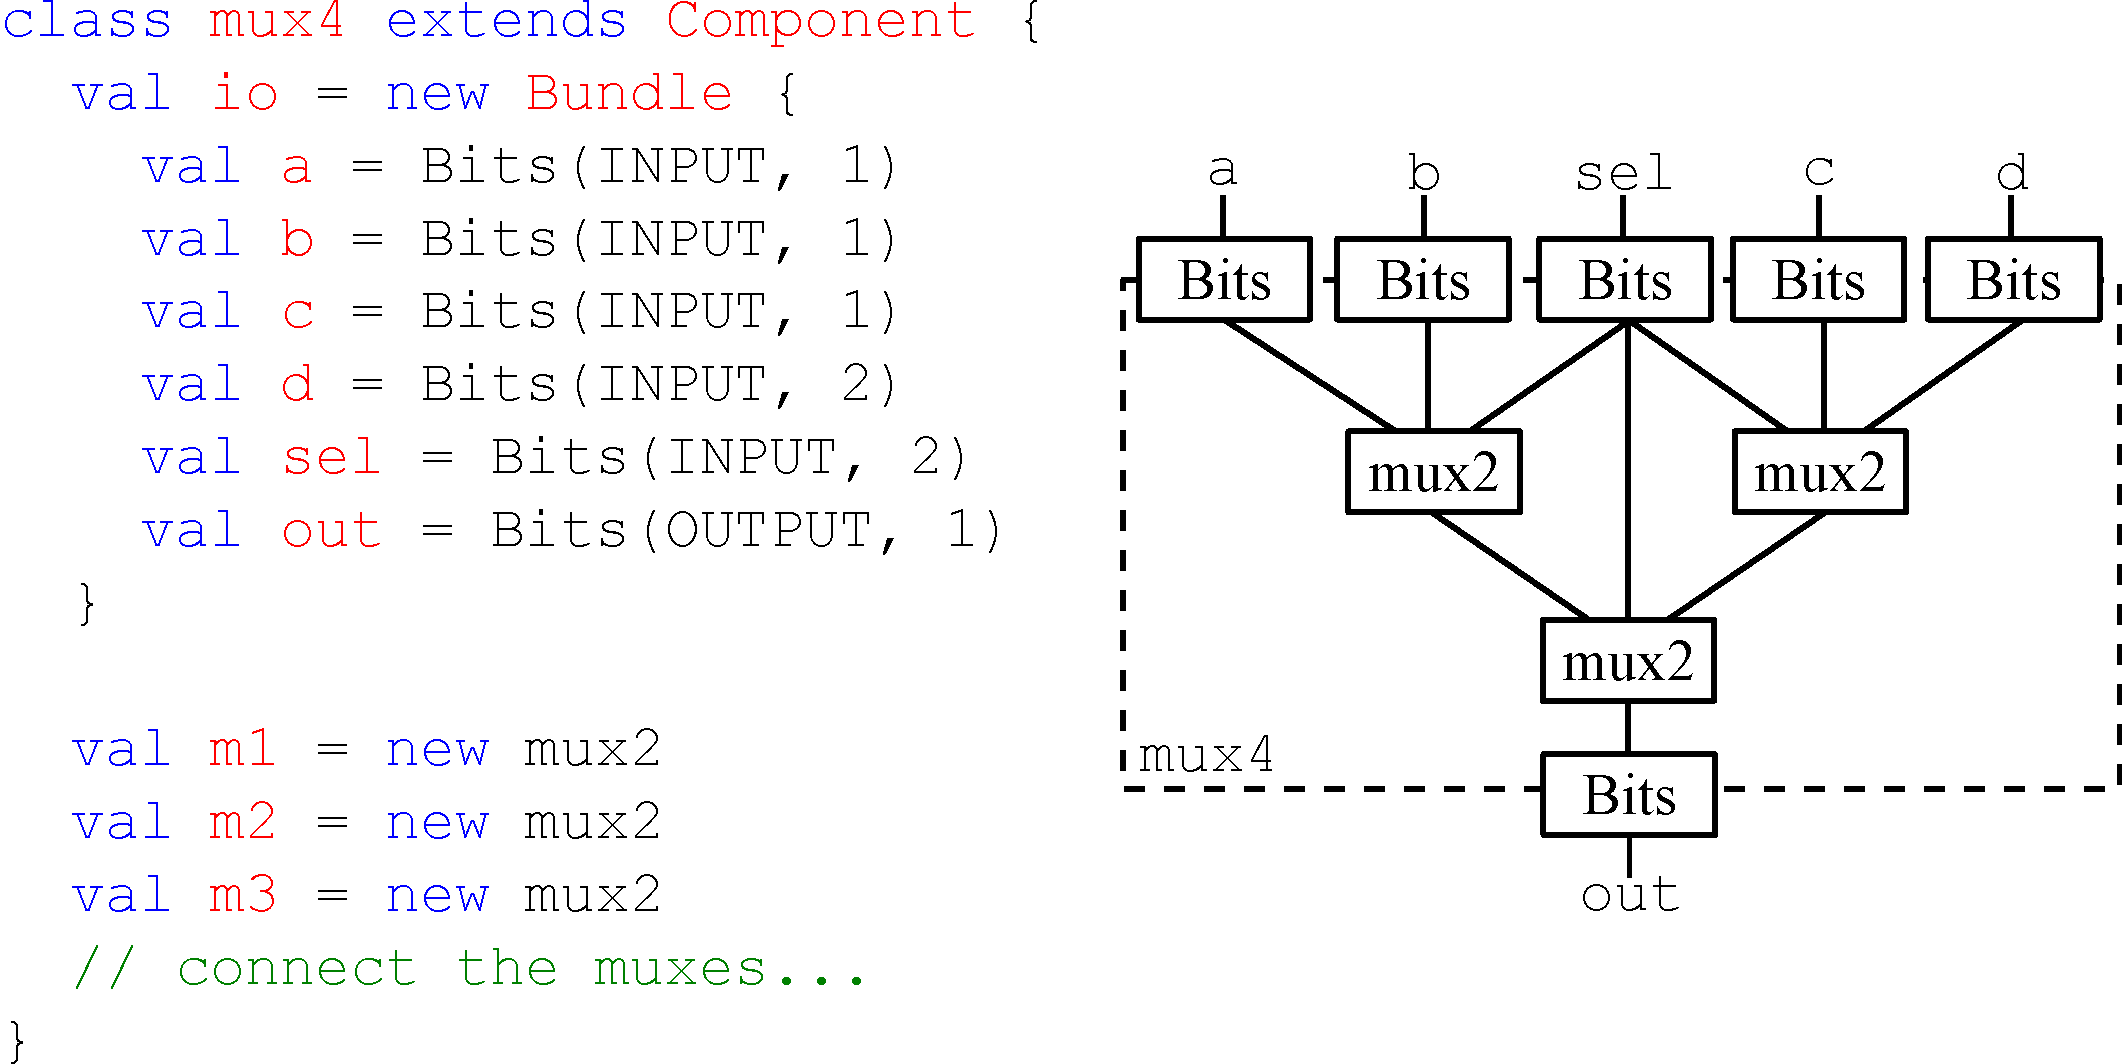
\includegraphics[width=\textwidth]{figures/mux4.pdf}
  \caption{4-Input Mux}
  \label{fig:mux4}
  \end{subfigure}
  \caption{Hierarchically building a 4-Input Mux out of 3 2-Input Muxes}
  \label{fig:muxcomp}
\end{figure}

{\bf Interfaces} When defining a new Component, users have to fill out
the {\tt io} field which is the input-output interface that
Components expose to each other. An input or output node in Chisel is
represented with a type {\tt Node} where the direction field is set to
either {\tt INPUT} or {\tt OUTPUT}. The example in
Figure~\ref{fig:mux} shows Component interfaces built out of {\tt
Bits} nodes. Input and output nodes can be
collected into Bundles, which are functionally similar to to C
structs, for better organization. 

{\bf Wiring} Once a Component's interface and circuit
implementation are defined, users will need to connect Components
together. Chisel provides two different ways for connecting
Components together. {\tt :=} is used for connections goings from
right to left while {\tt <>} is used for connections that go in either
direction. Both connection operators can be used to connect either individual
ports or entire Bundles. If used for the latter, the connection
operator will recursively walk through Bundle and wire each element
individually.

\subsection{Backend}
The Backend takes as input a directed graph of {\tt Nodes} and
generates code for the specified backend. Figure~\ref{fig:backend}
shows how Chisel's backend generates code from a directed graph of
nodes. Chisel currently generates code for two backends: Verilog and C++.

{\bf Elaboration} The elaboration phase performs backend specific
transformation on the graph in order to generate valid code for that
backend. For example, it is desirable to preserve Component hierarchy
when targeting the Verilog backend, so the elaboration phase will do a
graph walk to match nodes into components. For the C++ backend, the
elaboration phase will transform the graph into a directed acyclic
graph and perform a topological sort.

The elaboration phase also performs transformations and checks that
are common to both backends such as width inference and combinational
loop detection.

\begin{figure}[!h]
\centering
  \begin{subfigure}[t]{0.48\textwidth}
  \centering
  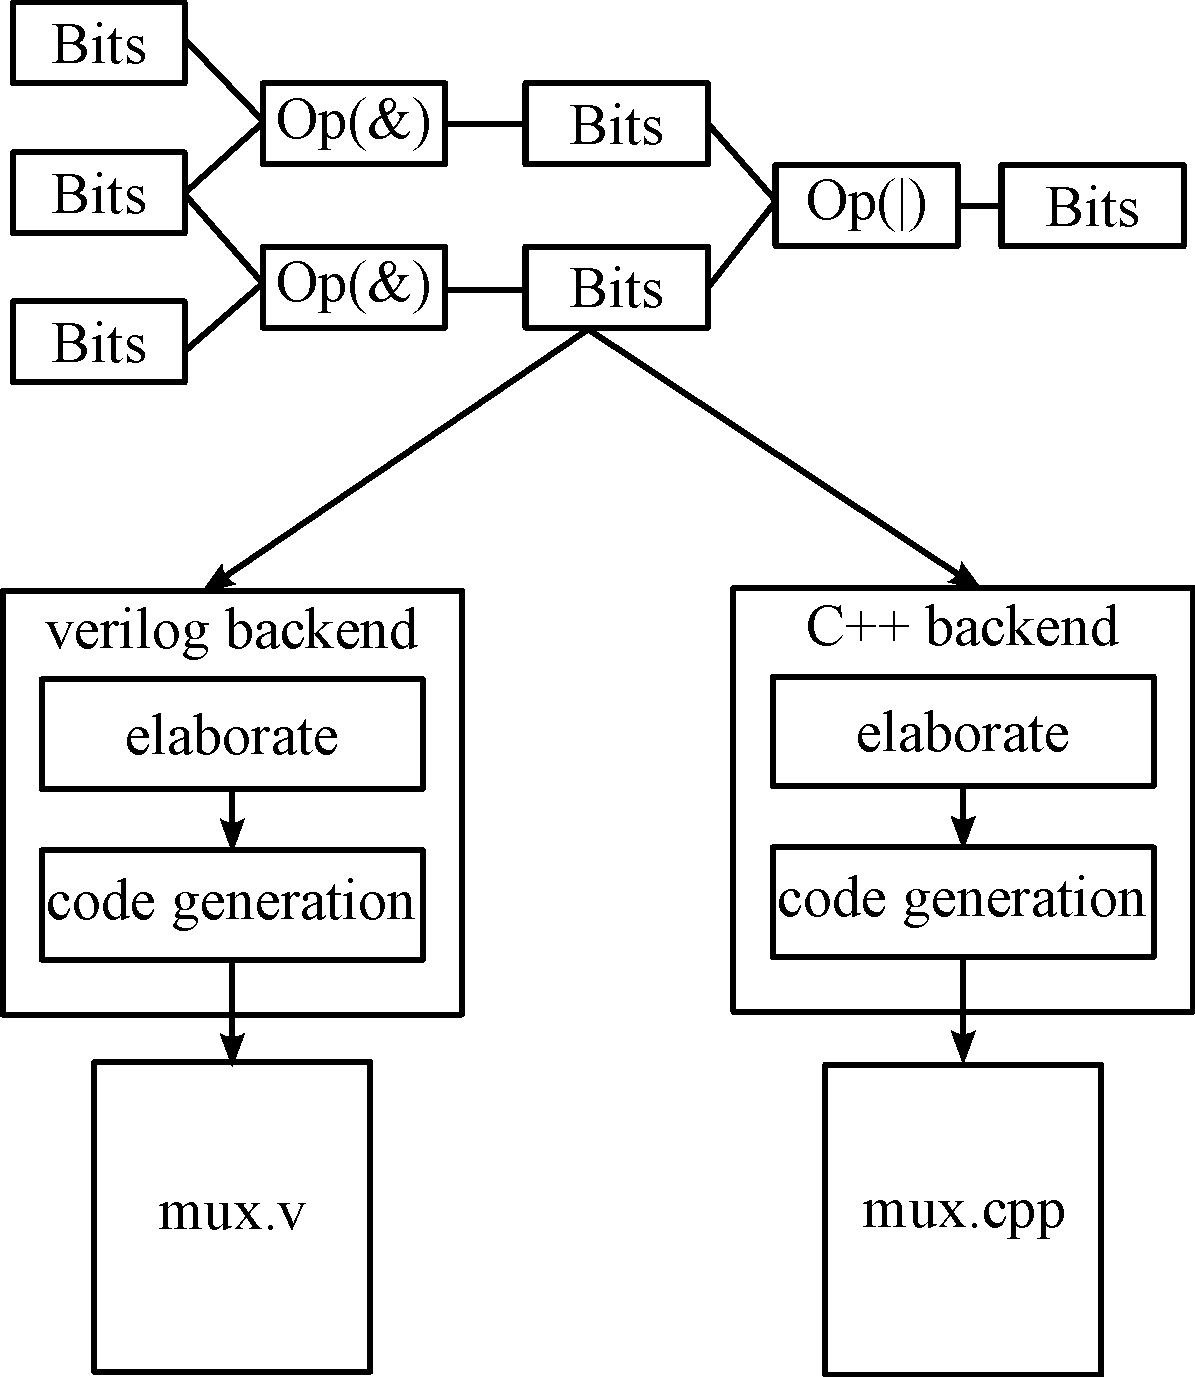
\includegraphics[width=0.7\textwidth]{figures/emit.pdf}
  \caption{Elaboration and Code Generation Process}
  \label{fig:emit}
  \end{subfigure}
  \hfill
  \begin{subfigure}[t]{0.48\textwidth}
  \centering
  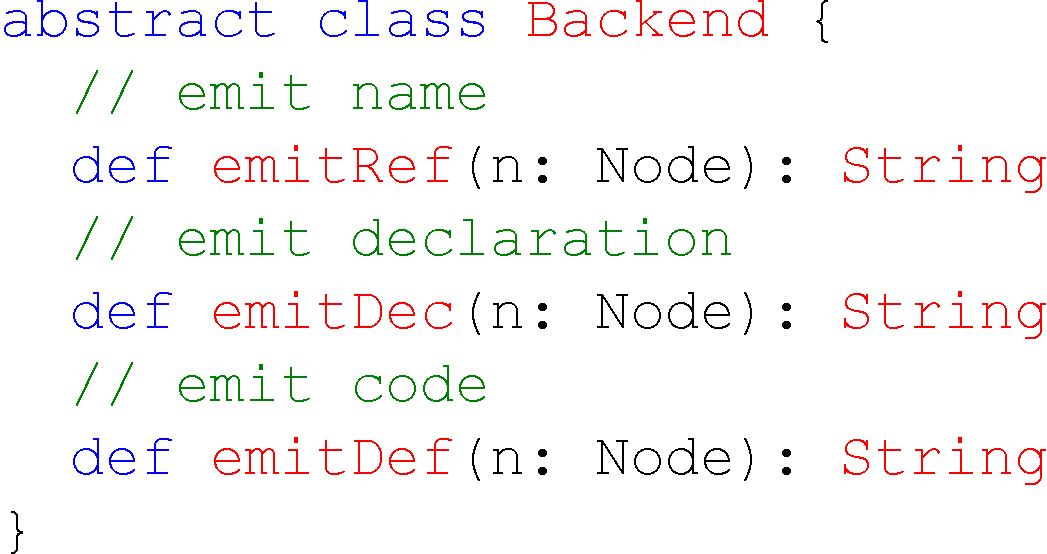
\includegraphics[width=\textwidth]{figures/backend.pdf}
  \caption{Backend API}
  \label{fig:backendapi}
  \end{subfigure}
\caption{Chisel Backend}
\label{fig:backend}
\end{figure}

{\bf Code Generation} Figure~\ref{fig:backendapi} shows the API for
generating code from an elaborated graph of nodes. The {\tt emitDec}
function is called to generate the code for declaring the node, {\tt
emitRef} is called to generate the reference to a node, and {\tt
emitDef} is called to generate the code. As an example, suppose the
Verilog backend is generating code for an {\tt Op} node that performs
an add. The {\tt emitDec} function, when called, returns the
string
\begin{align*}
\centering
\text{\tt{wire [31:0] a;}}
\end{align*}
assuming that the {\tt Op} is 32-bits wide and its user assigned name
is {\tt a}. The {\tt emitDef} function, when called, returns the
string
\begin{align*}
\centering
\text{\tt{assign a = b + c;}}
\end{align*}
assuming that the two nodes in the {\tt Op}'s input list have names
{\tt b} and {\tt c}.

\cite{Bachrach:2012}
